\section{Hardware}\label{sect:hardware}

We have three machines equipped with a CUDA compatible graphics card. This section will list the specifications of the machines and discuss the implications of writing code for different specifications.

Our hardware specifications can be seen in table \ref{table:hardware}. All benchmarks seen so far have been made on machine 2. 

Specifications of the graphic cards were found on \cite{techpowerup:gpu_specs}. The specifications for L1 Cache and L2 Cache refer to the GPU's cache. The clock speeds are approximate, since they have both a base clock speed and boost clock speed, and they may speed up and down, depending on power availability and temperature.

\begin{table}[h]
\caption{Our hardware specifications for our 3 machines.}
\label{table:hardware}
\begin{adjustbox}{width=\columnwidth,center}
\begin{tabular}{rlll}
 & \multicolumn{1}{c}{\textbf{Machine 1}}  & \multicolumn{1}{c}{\textbf{Machine 2}}      & \multicolumn{1}{c}{{\color[HTML]{000000} \textbf{Machine 3}}} \\ \Cline{2-4}{3.0pt} 
\multicolumn{1}{r|}{\textbf{CPU}}               & \multicolumn{1}{l|}{AMD Ryzen 7 5800X}  & \multicolumn{1}{l|}{AMD Ryzen 5600H}        & \multicolumn{1}{l|}{AMD Ryzen 7 5800HS}                       \\\cline{2-4} 
\multicolumn{1}{r|}{\textbf{RAM}}               & \multicolumn{1}{l|}{64 GB}              & \multicolumn{1}{l|}{16 GB}                  & \multicolumn{1}{l|}{16 GB}                                    \\ \Cline{2-4}{3.0pt}
\multicolumn{1}{r|}{\textbf{GPU}}               & \multicolumn{1}{l|}{NVIDIA RTX 4070 TI} & \multicolumn{1}{l|}{NVIDIA RTX 3060 Mobile} & \multicolumn{1}{l|}{NVIDIA GeForce MX450}                     \\ \cline{2-4} 
\multicolumn{1}{r|}{\textbf{VRAM}}              & \multicolumn{1}{l|}{12 GB}              & \multicolumn{1}{l|}{6 GB}                   & \multicolumn{1}{l|}{2 GB}                                     \\ \cline{2-4} 
\multicolumn{1}{r|}{\textbf{CUDA Cores}}   & \multicolumn{1}{l|}{7680}               & \multicolumn{1}{l|}{3840}                   & \multicolumn{1}{l|}{896}                                      \\ \cline{2-4} 
\multicolumn{1}{r|}{\textbf{Average Clock Speed}}          & \multicolumn{1}{l|}{$\sim$2400 MHz}                 & \multicolumn{1}{l|}{$\sim$1100 MHz}                     & \multicolumn{1}{l|}{$\sim$1100 MHz}                                       \\ \cline{2-4}
\multicolumn{1}{r|}{\textbf{Memory Clock Speed}}          & \multicolumn{1}{l|}{1313 MHz}                 & \multicolumn{1}{l|}{1750 MHz}                     & \multicolumn{1}{l|}{1250 MHz}                                       \\ \cline{2-4}
\multicolumn{1}{r|}{\textbf{SM Count}}          & \multicolumn{1}{l|}{60}                 & \multicolumn{1}{l|}{30}                     & \multicolumn{1}{l|}{14}                                       \\ \cline{2-4} 
\multicolumn{1}{r|}{\textbf{L1 Cache}}          & \multicolumn{1}{l|}{128 KB (per SM)}    & \multicolumn{1}{l|}{128 KB (per SM)}        & \multicolumn{1}{l|}{64 KB (per SM)}                           \\ \cline{2-4} 
\multicolumn{1}{r|}{\textbf{L2 Cache}}          & \multicolumn{1}{l|}{48 MB}              & \multicolumn{1}{l|}{3 MB}                   & \multicolumn{1}{l|}{512 KB}                                   \\ \Cline{2-4}{3.0pt}
\end{tabular}
\end{adjustbox}
\end{table}

Every SM has access to 128 cores on both machine 1 and machine 2.\footnote{Because: Cores per SM = Total cores / SM Count} Machine 1 has double the amount of cores as machine 2 and also double the amount of SMs. Machine 1 also have about double the clock speed as machine 2 and 3, enabling twice as many instructions to be processed. In theory, this would allow machine 1 to perform four times as many GPU operations at once as machine 2.

Machine 2 has about 4 times as many cores as machine 3, but only double the amount of SMs. So on machine 3, each SM has access to 64 cores. This is further reflected in the fact that the L1 cache for each of the 3 machines have exactly one KB per core an SM have access to. In theory, each SM on machine 1 and machine 2 can do double the amount of work that an SM can on machine 3. They have about the same clock speed. Further, machine 2 can do double the amount of work than machine 3, since it has double the amount of SMs. This means machine 2 can do 4 times as much work as machine 3. By transitivity machine 1 can do double that, so 16 times as much work as machine 3.

These performance gains all rely on code that is \textit{highly} optimized for each machine. In contrast, we strive to write portable code that runs well on all our machines. This goal also aligns with the purpose of CUDA as stated in \cite[Section 1.3]{nvidia:cudadoc}.

To see if our code achieves near these potential performance increases, we ran the benchmarks for the fastest parallel implementations of each algorithm. Figure \ref{fig:diagrams for all three algorithms} shows the running times of all three machines compared to each other for the largest matrix we benchmark on. The full benchmarks for all sizes can be seen in figures 

\begin{figure}[ht]
     \centering
     \begin{subfigure}[b]{0.32\textwidth}
         \centering
         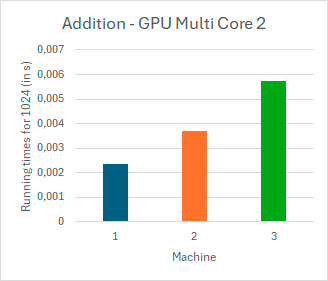
\includegraphics[width=\textwidth]{Documents/Report/Figures/Addition.png}
         \label{fig:addition diagram}
     \end{subfigure}
     \hfill
     \begin{subfigure}[b]{0.32\textwidth}
         \centering
         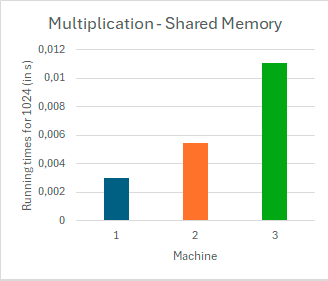
\includegraphics[width=\textwidth]{Documents/Report/Figures/Multiplication.png}
         \label{fig:multiplication diagram}
     \end{subfigure}
     \hfill
     \begin{subfigure}[b]{0.32\textwidth}
         \centering
         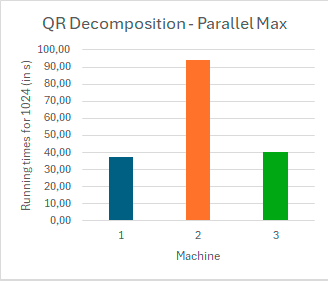
\includegraphics[width=\textwidth]{Documents/Report/Figures/QR.png}
         \label{fig:}
     \end{subfigure}
        \caption{Running times for matrices with side length 1024 on our three machines.}
        \label{fig:diagrams for all three algorithms}
\end{figure}

 With addition, it can be seen that machine 1 has about